\documentclass[12pt,a4paper]{article}
\usepackage[utf8]{inputenc}
\usepackage[spanish]{babel}
\usepackage{amsmath}
\usepackage{amsfonts}
\usepackage{amssymb}
\usepackage{graphicx}
\usepackage[left=2cm,right=2cm,top=2cm,bottom=2cm]{geometry}

%--------------------------------------------------------%
%         Paquetes usados sólo para esta entrega         %
%--------------------------------------------------------%

\usepackage[hidelinks]{hyperref}
\usepackage{algorithm}
\usepackage{algorithmic}
\usepackage{float}




\author{Ignacio Aguilera Martos \\
	DNI: 77448262V       e-mail: nacheteam@correo.ugr.es}
\title{Mejorando The Whale Optimization Algorithm \\ Metaheurísticas}
\date{Curso 2017-2018}

%Quita la sangría
\setlength{\parindent}{0cm}


\begin{document}
	\maketitle

	\tableofcontents

	\newpage

	%p 56

%	\framebox[16cm][c]{\LaTeX}

	\section{Introducción del problema}
	\label{sec:introProblema}
	
		Durante este trabajo he tenido como objetivo desarrollar un algoritmo mejorado a partir de un algoritmo bioinspirado de partida. Este algoritmo ha sido 'The Whale Optimization Algorithm' desarrollado y estudiado por los investigadores Seyedali Mirjalili y Andrew Lewis ambos de la universidad de Griffith.
		
		Para la comparativa y estudio de los resultados hemos puesto nuestro algoritmo a calcular los mínimos de 20 funciones. Estas funciones son las mismas que se utilizaron en la competición CEC2014, competición que pasaré a comentar brevemente en la siguente sección.
	
	\subsection{Competición CEC2014}
	
		Esta competición es un referente a nivel mundial en cuanto a competiciones de algoritmos se refiere. La intención de la competición es poner todos los algoritmos a ejecutar con diferentes dimensiones: 10,30,100,... de forma que se puedan comparar a posteriori los resultados obtenidos por los mismos.
		
		El problema consiste en minimizar 30 funciones que a priori no tienen un mínimo fácilmente localizable, como única garantía se tiene que el mínimo está localizado en el compacto $[-100,100]^n$ donde n es la dimensión considerada.
		
		En esta competición del año 2014 se evaluaron las funciones en dimensión 10,30,50 y 100 pero en este trabajo sólo hemos abarcado el problema de dimensión 10 y 30. Además cabe destacar que el algoritmo ganador en la competición fue L-SHADE.
	
	\subsection{Módulo de funciones CEC2014}
	
		Para poder ejecutar el algoritmo diseñado sobre las funciones de la competición CEC2014 primero tenemos que tener una implementación de las mismas. Mi decisión fue utilizar Python para el desarrollo del algoritmo, por la rapidez y facilidad en la escritura y sintaxis y por disponer de bibliotecas muy potentes en las que poder apoyar mi código.
	
		La implementación de las funciones nos fue dada en C++, por lo que tuve que hacer un módulo en Python primero que importase las funciones de C++ para poder utilizarlas en Python. Este trabajo lo hice de forma conjunta con mi compañero Pablo Baeyens utilizando la biblioteca Cython. Tras esto implementamos dos interfaces muy sencillas que permiten ejecutar las primeras 20 funciones de la competición a través de una clase Benchmark.
		
		Cabe destacar que esta idea se me ocurrió tras ver que el profesor de la Universidad de Granada en Ceuta Daniel Molina había desarrollado un módulo parecido para la competición de 2013 \cite{danielMolinaCEC2013}. Tras contactar con el y apoyarnos en su código terminamos de desarrollar el módulo de las funciones y lo subimos a GitHub dejándolo a disposición del resto de alumnos junto con el código de otro compañero que realizó el mismo trabajo para el lenguaje Julia \cite{cec2014github}.

	\newpage

	\section{Descripción del algoritmo inicial}
	\label{sec:descripcionAlgoritmoInicial}
	
		En esta sección vamos a pasar a describir con detalle el algoritmo inicial propuesto por Mirjalili y Lewis en su artículo \cite{paperWOA} desgranando cada elemento que pueda resultar interesante para el desarrollo de la explicación de las siguientes versiones.
	
	\subsection{Inspiración en la ballena jorobada}
	
		Este algoritmo basa su comportamiento en la naturaleza, por lo que es uno de los llamados algoritmos bioinspirados. En concreto en este caso el algoritmo toma como idea la forma en que las ballenas jorobadas se aproximan a su comida.
		
		Estas ballenas tienen dos formas comunes de alimentarse: aletear sobre sus presas y después comérselas o realizar un camino ascendente hacia ellas en forma de espiral para así concentrar los peces en la parte superior de la misma mientras que expulsan burbujas para aturdir a sus presas.
		
		Mediante estas dos formas de caza se están describiendo dos formas de aproximarse hacia las presas que en nuestro caso serán dos soluciones, por lo que con esto tendremos una aproximación lineal hacia la solución lo que nos va a dar en teoría una buena convergencia y tendremos una aproximación en espiral que intentará que no nos quedemos encerrados en mínimos locales ya que estaremos explorando un entorno de la solución cada vez más pequeño.
	
	\subsection{Modelo matemático}
	
		Para la descripción del modelo vamos a definir $a\in \mathbb{R}$ como un número que se decrementa de forma lineal desde 2 hasta 0 y $r\in \mathbb{R}$ un vector aleatorio en el intervalo $[0,1]$.
		
		A partir de estos números reales podemos definir $C\in \mathbb{R}$ como $C=2\cdot r$ y $A \in \mathbb{R}$ como $A = 2\cdot a \cdot r - a$. Nótese que estas variables van dependiendo de los dos reales definidos previamente.
		
		Para el movimiento lineal vamos a definir $D\in \mathbb{R}$ como $D=|C\cdot X^*(t)-X(t)|$ donde $X^*(t)$ es la posición de la mejor solución hallada hasta el momento y $X(t)$ es la posición actual de la ballena.
		
		Para el movimiento lineal con lo definido si estamos en la iteración t entonces obtenemos la posición de la siguiente iteración como:
		
		$$X(t+1) = X^*(t)-A\cdot D$$
		
		Donde el producto entre vectores se refiere al producto elemento por elemento y el producto de escalar por vector es el definido en un espacio vectorial cualquiera.
		
		Esta aproximación hecha hasta el momento es la lineal, la cual es la más sencilla de las dos y nos da el comportamiento más simple. Ahora vamos a desarrollar el movimiento espiral.
		
		Si nos fijamos en la variable A podemos ver que en realidad es un valor aleatorio en el intervalo $[-a,a]$ lo que nos permite que en cada iteración podamos tomas como siguiente punto cualquiera de los que se encuentran en el segmento que une $X(t)$ con $X^*(t)$.
		
		Para la aproximación en espiral definimos la constante real $b\in \mathbb{R}$ que que nos da la forma concreta de la espiral, en el caso del algoritmo implementado para el paper $b=1$. También definimos la variable $l\in \mathbb{R}$ que es un valor aleatorio en el intervalo $[-1,1]$.
		
		En este caso definimos también una variable dependiente de la posición actual y la mejor hasta el momento $D'\in \mathbb{R}$ como $D' = |X^*(t)-X(t)|$.
		
		Con todo lo definido la expresión del movimiento en espiral para la siguiente iteración t+1 viene dada por:
		
		$$X(t+1) = D'\cdot e^{bl}\cdot \cos(2\pi l) + X^*(t)$$
		
		Tras esto ya tenemos definidos los dos tipos de movimientos con las ecuaciones que los modelan. El comportamiento real del algoritmo va a depender de un valor aleatorio $p\in [0,1]$ de forma que:
		
		$$X(t+1) = 
		\begin{cases}
			X^*(t)-A\cdot D & si \ p<0.5\\
			D'\cdot e^{bl}\cdot \cos(2\pi l)+X^*(t) & si \ p\geq0.5
		\end{cases}$$
		
		A esto le sumamos el hecho de que en un estado inicial del algoritmo, o lo que es lo mismo si $|A|>1$, tenemos que en vez de dirigirnos hacia la mejor ballena hasta el momento nos vamos a dirigir a una posición aleatoria, de forma que vamos a ensalzar la exploración sobre la convergencia. Todas las fórmulas permanecen igual salvo que $X^*$ en este caso es un $X_{rand}$ aleatorio.
		
		\begin{figure}[!h]
			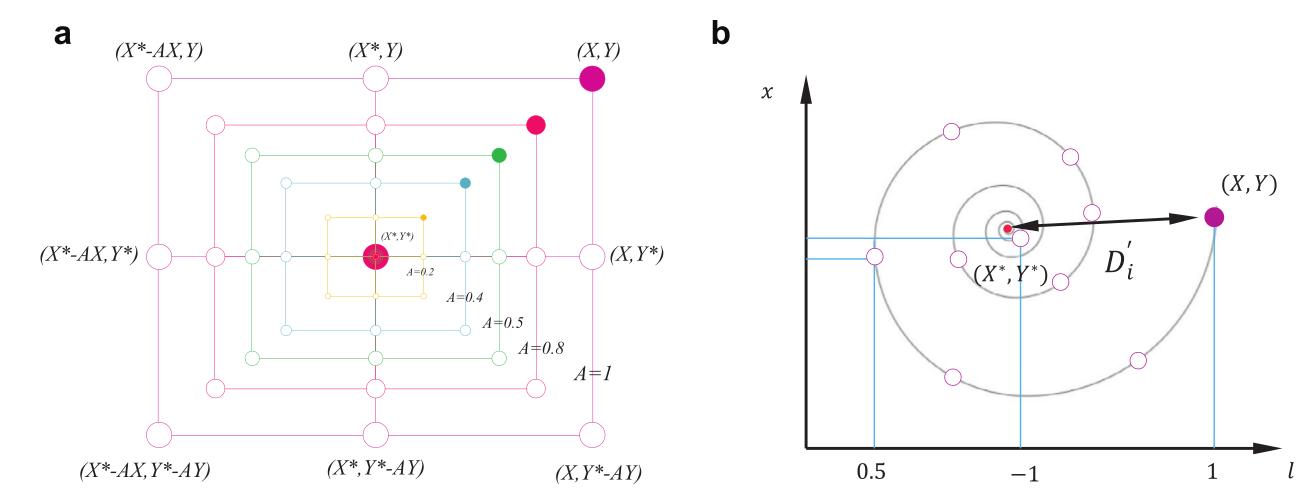
\includegraphics[scale=0.35]{./Imagenes/lineal_espiral.png}
			\caption{a) Aproximación lineal. b) Aproximación en espiral.}
		\end{figure}
		
	\subsection{Pseudocódigo del algoritmo}
	
	\section{Desarrollo de mejoras}
	\label{sec:desarrolloMejoras}
	
	\section{Versión final}
	\label{sec:versionFinal}
	
	\section{Resultados}
	\label{sec:resultados}
	
	%---------------------------------------------------------------------------------%
	
	%                               Bibliografía                                      %
	
	%---------------------------------------------------------------------------------%
	
	\newpage
	
	\bibliography{referencias} %archivo referencias.bib que contiene las entradas 
	\bibliographystyle{plain} % hay varias formas de citar

\end{document}
